

\section{Network Requirements and Structure}

A network both defines the composition advected by the hydro code as
well as describes the burning processes between those isotopes.
Evolving the species in a network requires an integrator.  The design
of \microphysics\ decouples the integrator from the network, allowing
for the ability to swap integrators as desired.  We discuss the
integrators in a later section.


At a minimum, a network needs to provide:
\begin{itemize}
 \item {\tt nspec} : the number of species in the network

 \item {\tt nspec\_evolve} : the number of species that are actually
   integrated in the network.  Usually this is {\tt nspec}, but in general
   any {\tt nspec\_evolve} $\le$ {\tt nspec} is allowed.  Those species
   not evolved are held constant in the integration.

   Note that the convention is that the first {\tt nspec\_evolve} out
   of the {\tt nspec} species are the ones evolved.

 \item {\tt naux} : the number of auxiliary quantities needed by the
   network (these are not evolved).  \MarginPar{does any net use these?}

 \item {\tt aion(:)} : the atomic weight (in atomic mass units) of the
   species

 \item {\tt zion(:)} : the atomic number of the species

 \item {\tt spec\_names(:)} : a descriptive name of the species
   (e.g. {\tt "hydrogen-1"})

 \item {\tt short\_spec\_names(:)} : a shorten version of the species name
   (e.g. {\tt "H1"})

 \item {\tt short\_aux\_names(:)} : the names of the auxiliary quantities

 \item {\tt network\_name} : a descriptive name for the network

\end{itemize}
Most of these quantities are Fortran parameters.

{\bf A convention adopted in \microphysics\ is that each network
is responsible for determining the energy release from a change
in composition}.  Most networks will provide an array of the species
binding energies and a routine to compute the energy yield from
the reaction rates.

There are three primary files within each network directory.

\begin{itemize}

\item {\tt actual\_network.f90}:

 This supplies the number and names of species and
auxiliary variables, as well as other initializing data, such as their
mass numbers, proton numbers, and binding energies. It needs to define
the {\tt nspec} and {\tt naux} quantities as integer parameters. Additionally
it must define {\tt nspec\_evolve}, the number of species that are actually evolved
during a burn; in most cases, this should have the same value as {\tt nspec}.
Finally, it must also define {\tt nrates}, the number of reaction rates
linking the isotopes in the network.

\item {\tt actual\_rhs.f90}:

This supplies an interface for computing the right-hand-side
of the network, the time-derivative of each species (and the temperature and
nuclear energy release), as well as the Jacobian. This is covered in more detail
in Chapter \ref{chapter:burners}.

\item {\tt actual\_burner.f90}:

This contains the interface for doing an actual burn.
In general, you will want to {\tt call integrator} to use one of the pre-defined
ODE integrators, but you could also write a custom integration here. This is
covered in more detail in Chapter \ref{chapter:burners}.

\end{itemize}

All three have initialization routines:
\begin{itemize}
  \item {\tt actual\_network\_init()}
  \item {\tt actual\_rhs\_init()}
  \item {\tt actual\_burner\_init()}
\end{itemize}
These must be called upon initialization. These should be not called
within OpenMP parallel regions, because in general they will modify
shared module data.

Note, depending on the network, some of these may do nothing, but
these interfaces are all required for maximum flexibility.


\section{Available Networks}


\subsection{{\tt aprox13}, {\tt aprox19}, and {\tt aprox21}}

These are alpha-chains (with some other nuclei) from Frank Timmes.
These networks share common rates (from {\tt Microphysics/rates}),
plasma neutrino loses (from {\tt Microphysics/neutrinos}), and
electron screening (from {\tt Microphysics/screening}).

\paragraph{Energy generation.} These networks store the total binding
energy of the nucleus in MeV as {\tt bion(:)}.  They then compute the
mass of each nucleus in grams as:
\begin{equation}
M_k = (A_k - Z_k) m_n + Z_k (m_p + m_e) - B_k
\end{equation}
where $m_n$, $m_p$, and $m_e$ are the neutron, proton, and electron
masses, $A_k$ and $Z_k$ are the atomic weight and number, and $B_k$
is the binding energy of the nucleus (converted to grams).  $M_k$
is stored as {\tt mion(:)} in the network.

The energy release per gram is converted from the rates as:
\begin{equation}
\edot = -N_A c^2 \sum_k \frac{dY_k}{dt} M_k - \edot_\nu
\end{equation}
where $N_A$ is Avogadro's number (to convert this to ``per gram'')
and $\edot_\nu$ is the neutrino loss term.

\subsection{{\tt breakout}}

\subsection{{\tt CONe2NSE}}

\subsection{{\tt general\_null}}

{\tt general\_null} is a bare interface for a nuclear reaction
network; no reactions are enabled, and no auxiliary variables are
accepted.  The data in the Fortran module is defined at compile type
by specifying an inputs file.  For example, {\tt
  Networks/general\_null/triple\_alpha\_plus\_o.net} would describe
the triple-$\alpha$ reaction converting helium into carbon, as well as
oxygen and iron.

At compile time, the network module {\tt actual\_network.f90}
is written using the python script {\tt write\_network.py}
and the template {\tt network.template}.  The {\tt make} rule
for this is contained in {\tt Make.package} (for \cpp\ \boxlib) and
{\tt GPackage.mak} (for F90 \boxlib).  The name of the inputs file
is specified by the variable {\tt GENERAL\_NET\_INPUTS}.

A version of this network comes with \maestro\ and \castro, so you do
not usually need to worry about the version in \microphysics.


\subsection{{\tt ignition\_chamulak}}

This network was introduced in our paper on convection in white dwarfs
as a model of Type Ia supernovae~\cite{wdconvect}.  It models
carbon burning in a regime appropriate for a simmering white dwarf,
and captures the effects of a much larger network by setting the ash
state and energetics to the values suggested in \cite{chamulak:2008}.

This network has {\tt nspec = 3}, but {\tt nspec\_evolve = 1}.  Only a
single reaction is modeled, converting \isot{C}{12} into ``{\tt
  ash}''.

\paragraph{Energy generation.} The binding energy, $q$, in this
network is interpolated based on the density.  It is stored as the
binding energy (ergs/g) {\em per nucleon}, with a sign convention that
binding energies are negative.  The energy generation rate is then:
\begin{equation}
\edot = q \frac{dX(\isotm{C}{12})}{dt} = q A_{\isotm{C}{12}} \frac{dY(\isotm{C}{12})}{dt}
\end{equation}
(this is positive since both $q$ and $dY/dt$ are negative)

\subsection{{\tt ignition\_reaclib}}

\subsection{{\tt ignition\_simple}}

This is the original network used in our white dwarf convection
studies~\cite{lowMach4}.  It includes a single-step
$^{12}\mathrm{C}(^{12}\mathrm{C},\gamma)^{24}\mathrm{Mg}$ reaction.
The carbon mass fraction equation appears as
\begin{equation}
\frac{D X(^{12}\mathrm{C})}{Dt} = - \frac{1}{12} \rho X(^{12}\mathrm{C})^2
    f_\mathrm{Coul} \left [N_A \left <\sigma v \right > \right]\enskip,
\end{equation}
where $N_A \left <\sigma v\right>$ is evaluated using the reaction
rate from (Caughlan and Fowler 1988).  The Coulomb screening factor,
$f_\mathrm{Coul}$, is evaluated using the general routine from the
Kepler stellar evolution code (Weaver 1978), which implements the work
of (Graboske 1973) for weak screening and the work of (Alastuey 1978
and Itoh 1979) for strong screening.


\subsection{{\tt iso7}}


\subsection{{\tt kpp}}


\subsection{{\tt powerlaw}}

This is a simple single-step reaction rate.
We will consider only two species, fuel, $f$, and ash, $a$, through
the reaction: $f + f \rightarrow a + \gamma$.  Baryon conservation
requres that $A_f = A_a/2$, and charge conservation requires that $Z_f
= Z_a/2$.  We take
our reaction rate to be a powerlaw in temperature.  The standard way
to write this is in terms of the number densities, in which case we
have
\begin{equation}
\frac{d n_f}{d t} = -2\frac{d n_a}{d t} = -r
\end{equation}
with
\begin{equation}
  r = r_0 n_X^2 \left( \frac{T}{T_0} \right )^\nu
\end{equation}
Here, $r_0$ sets the overall rate, with units of
$[\mathrm{cm^3~s^{-1}}]$, $T_0$ is a reference temperature scale, and
$\nu$ is the temperature exponent, which will play a role in setting
the reaction zone thickness.  In terms of mass fractions, $n_f = \rho
X_a / (A_a m_u)$, our rate equation is
\begin{eqnarray}
 \frac{dX_f}{dt} &=& - \frac{r_0}{m_u} \rho X_f^2 \frac{1}{A_f} \left (\frac{T}{T_0}\right)^\nu \equiv \omegadot_f \label{eq:Xf} \\
 \frac{dX_a}{dt} &=& \frac{1}{2}\frac{r_0}{m_u} \rho X_f^2 \frac{A_a}{A_f^2} \left (\frac{T}{T_0}\right)^\nu = \frac{r_0}{m_u} \rho X_f^2 \frac{1}{A_f} \left (\frac{T}{T_0}\right)^\nu  \label{eq:Xa}
\end{eqnarray}
We define a new rate constant, $\rt$ with units of $[\mathrm{s^{-1}}]$ as
\begin{equation}
\rt =  \begin{cases}
  \dfrac{r_0}{m_u A_f} \rho_0 & \text{if $T \ge T_a$} \\[1em]
  0                          & \text{if $T < T_a$}
 \end{cases}
\end{equation}
where $\rho_0$ is a reference density and $T_a$ is an activation
temperature, and then our mass fraction equation is:
\begin{equation}
\frac{dX_f}{dt} = -\rt X_f^2 \left (\frac{\rho}{\rho_0} \right ) \left ( \frac{T}{T_0}\right )^\nu
\end{equation}
Finally, for the
energy generation, we take our reaction to release a specific energy,
$[\mathrm{erg~g^{-1}}]$, of $\qburn$, and our energy source is
\begin{equation}
\epsdot = -\qburn \frac{dX_f}{dt}
\end{equation}

There are a number of parameters we use to control the constants in
this network.  This is one of the few networks that was designed
to work with {\tt gamma\_law\_general} as the EOS.

\subsection{{\tt rprox}}

This network contains 10 species, approximating hot CNO,
triple-$\alpha$, and rp-breakout burning up through \isot{Ni}{56},
using the ideas from \cite{wallacewoosley:1981}, but with modern
reaction rates from {\sf ReacLib}~\cite{ReacLib} where available.
This network was used for the X-ray burst studies in
\cite{xrb:II,xrb:III}, and more details are contained in those papers.


\subsection{{\tt triple\_alpha\_plus\_cago}}

This is a 2 reaction network for helium burning, capturing the $3$-$\alpha$
reaction and $\isotm{C}{12}(\alpha,\gamma)\isotm{O}{16}$.  Additionally,
\isot{Fe}{56} is included as an inert species.

This network has {\tt nspec = 4}, but {\tt nspec\_evolve = 3}.



\subsection{{\tt xrb\_simple}}



\section{Reaction ODE System}

The equations we integrate to do a nuclear burn are:
\begin{eqnarray}
  \frac{dY_k}{dt} &=& \omegadot_k(\rho,Y_k,T), \label{eq:spec_integrate} \\
  \frac{de}{dt} &=& \sum_k \xi_k A_k \dot{Y}_k \label{eq:enuc_integrate} \\
  \frac{dT}{dt} &=&\frac{\dot{e}}{c_x}. \label{eq:temp_integrate}
\end{eqnarray}
$Y_k \equiv X_k / A_k$ is the molar fraction of species $k$, where
$X_k$ is the mass fraction and $A_k$ is the mass number of that species.
$e$ is the internal energy, $T$ is the temperature\footnote{Note that in
previous versions of our networks in \castro\ and \maestro,
there was another term in the temperature equation relating to the
chemical potential of the gas as it came from the EOS. We have since
decided that this term should analytically cancel to zero in all cases
for our nuclear networks, and so we no longer think it is correct to
include a numerical approximation of it in the integration scheme. So
the current results given by our networks will in general be a little
different than in the past.}
, and $c_x$ is the specific heat for the fluid. $\xi_k$ is the energy
release associated with the destruction of species $k$; normally it
is given by the (absolute value of the) binding energy for that species.

{\bf Note that while $Y_k$ is the integration variable, this is invisible to
the code that calls the burner---it hands the burner the mass fractions $X_k$
and gets back updated mass fractions.}


While this is the most common way to construct the set of
burn equations, and is used in most of our production networks,
all of them are ultimately implemented by the network itself, which
can choose to disable the evolution of any of these equations by
setting the RHS to zero. The integration software provides some
helper routines that construct common RHS evaluations, like the RHS
of the temperature equation given $\dot{e}$, but these calls
are always explicitly done by the individual networks rather than
being handled by the integration backend. This allows you to write a
new network that defines the RHS in whatever way you like.

We integrate these using a stiff ordinary differential equation
integration solver. The absolute error tolerances are set by default
to $10^{-12}$ for the species, and a relative tolerance of $10^{-6}$
is used for the temperature and energy.  The integration
yields the new values of the mass fractions, $Y_k^\outp$.

\subsection{Disabling $T$ Evolution}


\subsection{{\tt nspec\_evolve} Implementation}


\subsection{Single Zone Burn Unit Tests}


\subsection{Burn Parameters}

The full set of parameters for the integration is listed in Chapter \ref{chapter:parameters}.
In this section we will explain the most relevant ones in more detail.
Remember that all of these are controlled by including them in your runtime
inputs (either with all other parameters in the standard inputs file for
MAESTRO, or the \texttt{extern} namelist of the probin file for CASTRO).

In evolving these equations, we need to evaluate $c$. This involves two
issues. First, we need to decide which specific heat we are talking about;
usually we deal with either the specific heat at constant pressure ($c_p$)
or the specific heat at constant volume ($c_v$). The EOS generally will
provide both of these specific heats; which one to use is a choice the user
needs to make based on the physics of their problem. It is controlled by the
parameter \texttt{do\_constant\_volume\_burn}, which will use $c_v$ if true
and $c_p$ is false. Second, a fully accurate integration of Equation
\ref{eq:temp_integrate} requires an evaluation of the specific heat at
each integration step, which involves an EOS call given the current temperature.
However, this may add significantly to the expense of the calculation,
especially for smaller networks where construction of the RHS is inexpensive,
and the user may decide that they are OK with a less accurate integration
(or they believe the specific heat won't change that much anyway during a burn).
This can be enabled or disabled with the parameter \texttt{call\_eos\_in\_rhs}.
A middle ground between fully on and fully off for this parameter is obtained
with the runtime parameter \texttt{dT\_crit}, which is the fractional change
needed in the temperature during a burn to trigger an EOS call that updates
the thermodynamic variables. Note that this is fully independent of
\texttt{call\_eos\_in\_rhs}. If you use this option, we do a crude prediction
of the specific heat in between EOS calls using a numerically constructed
approximation to the temperature derivative of the specific heat.

The \texttt{renormalize\_abundances} parameter controls whether we renormalize
the abundances so that the mass fractions sum to one during a burn. This
has the positive benefit that in some cases it can prevent the integrator
from going off to infinity or otherwise go crazy; a possible negative benefit
is that it may slow down convergence because it interferes with the integration
scheme. Regardless of whether you enable this, we will always ensure that the
mass fractions stay positive and larger than some floor \texttt{small\_x}.

While we normally evolve all of these equations simultaneously, which is
usually called a ``self-heating'' burn because the temperature is allowed
to respond to the reactions as they occur, it is
sometimes the case that you do not want to update the temperature at all
during the burn -- this is a so-called ``hydrostatic'' burn. You can
set the RHS of the temperature equation to zero by setting
\texttt{burning\_mode = 0}. We also offer the ``hybrid'' burn approach
(\texttt{burning\_mode = 2}) introduced by \cite{raskin:2010}, which
does a hydrostatic burn, but recomputes a self-heating burn if the
final energy release from the hydrostatic burn was negative (the
logic being that a negative energy release corresponds to NSE conditions).

The integration tolerances for the burn are controlled by \texttt{rtol\_spec},
\texttt{rtol\_enuc}, and \texttt{rtol\_temp}, which are the relative error
tolerances for Equations \ref{eq:spec_integrate}, \ref{eq:enuc_integrate},
and \ref{eq:temp_integrate}, respectively. There are corresponding \texttt{atol}
parameters for the absolute error tolerances. Note that not all integrators
handle error tolerances the same way; see Section \ref{sec:stiff_solvers} for
notes on any differences between them.

\section{Stiff ODE Solvers}
\label{sec:stiff_solvers}

Let's turn to the set of options we have for evolving our system of coupled,
stiff ODEs. You can control which integrator you use by setting the
\texttt{INTEGRATOR\_DIR} variable in your makefile equal to the name of
one of the following integrators from the list (this corresponds to the
directory names in \texttt{integrators/}).

\subsection{VODE}
\label{sec:VODE}

\subsection{VBDF}
\label{sec:VBDF}

\subsection{BS}
\label{sec:BS}


\begin{sidewaysfigure}
\centering
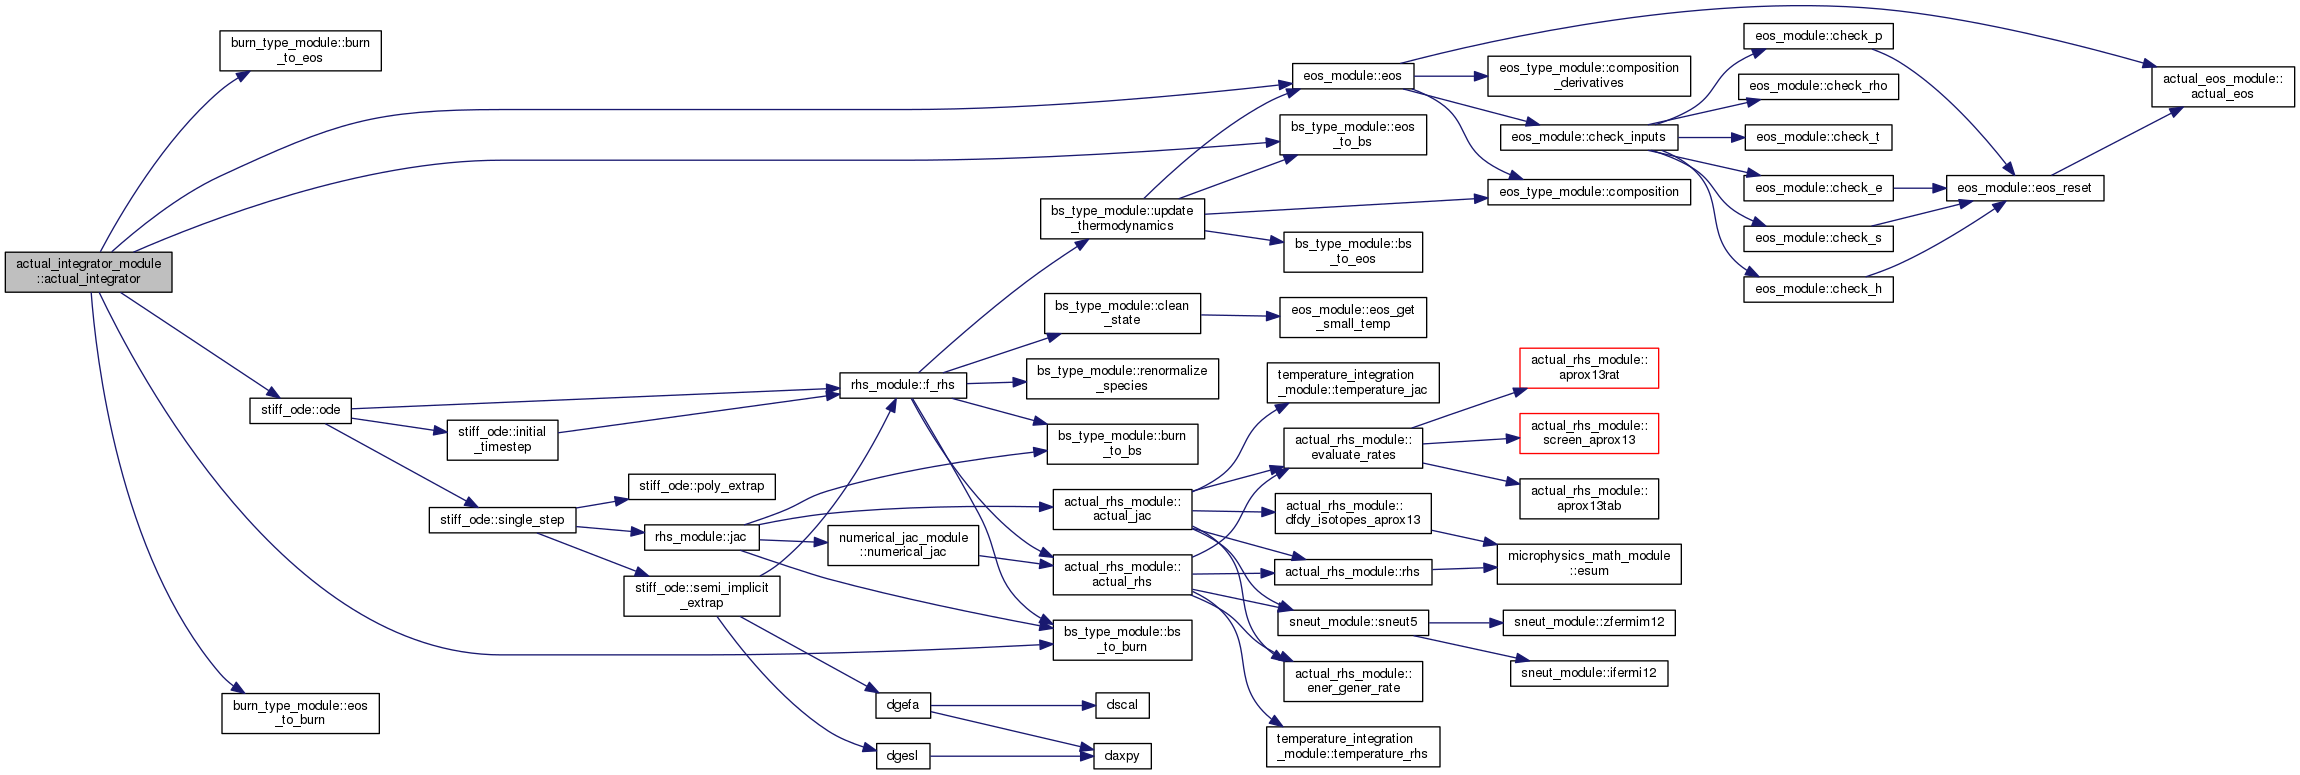
\includegraphics[width=\linewidth]{doxygen_network}
\end{sidewaysfigure}
